\documentclass[a4paper,14pt]{extreport}

\usepackage[utf8]{inputenc} % Set Encoding
\usepackage[T1]{fontenc} % Enable cyrillic fonts
\usepackage{fontspec} % Using custom fonts (requires -xelatex flag)
\usepackage{ifplatform} % Cross platform
\usepackage[russian,english,ukrainian]{babel} % Using languages
\usepackage{geometry} % Set margins
\usepackage{titlesec} % For section modification
\usepackage{indentfirst} % Inserts indents in paragraphs
\usepackage{minted} % For code listing
\usepackage{graphicx} % For image insertions
\usepackage{float} % For positioning
\usepackage[section]{placeins}
\usepackage{fancyhdr}
\usepackage{caption}
\usepackage{dirtytalk}
\usepackage{enumitem} % List indents
\usepackage{chngcntr}
\usepackage[english]{babel}
\usepackage[nottoc]{tocbibind}
\usepackage{color}
\usepackage{xpatch}
\definecolor{spot}{rgb}{0,0.2,0.6}
\usepackage[colorlinks,allcolors=spot,bookmarksopen=true,pdfstartview=FitH]{hyperref}

\counterwithout{section}{chapter}

\pagestyle{fancy}

\fancyhf{}
\fancyhead[R]{\thepage}
\renewcommand{\headrulewidth}{0pt}
\fancyheadoffset{0mm}
\fancyfootoffset{0mm}
\renewcommand{\headrulewidth}{0pt}
\renewcommand{\footrulewidth}{0pt}

\fancypagestyle{plain}{
    \fancyhf{}
    \rhead{\thepage}}


\pagenumbering{gobble}

\usemintedstyle{bw}

\geometry{
  a4paper,
  left=30mm,
  right=20mm,
  top=20mm,
  bottom=20mm
}

\DeclareCaptionLabelFormat{gostfigure}{Рисунок #2}
\DeclareCaptionLabelFormat{gosttable}{Таблиця #2}
\DeclareCaptionLabelSeparator{gost}{~---~}
\captionsetup{labelsep=gost}
\captionsetup[figure]{labelformat=gostfigure, justification=centering,
labelsep=gost}
\captionsetup[table]{labelformat=gosttable, labelsep=gost}

\setlength\parindent{2.5em}
\renewcommand{\baselinestretch}{2.0}
\linespread{1.3} % Set default line spacing

\iflinux
\setmainfont{Liberation Serif} % Set default font on Linux
\fi
\ifwindows
\setmainfont{Times New Roman} % Set default font on Windows
\fi

\titleformat{\section}
{\normalfont}{\thesection}{1em}{}

\titleformat{\subsection}
{\normalfont}{\thesubsection}{1em}{}

\titleformat{\subsubsection}
{\normalfont}{\thesubsubsection}{1em}{}

\titleformat{\chapter}[block]
    {\filcenter\bfseries}
    {\thechapter}
    {1em}
    {\MakeUppercase}{}

\renewcommand{\headrulewidth}{0pt}

\titlespacing{\chapter}{0pt}{-30pt}{2em}
\titlespacing\section{0cm}{2em}{1ex}
\titlespacing\subsection{0cm}{1ex}{1ex}

\newcommand\chap[1]{%
  \chapter*{#1}%
  \addcontentsline{toc}{chapter}{\uppercase{#1}}}

\graphicspath{{./screens}}

\setlist[enumerate]{leftmargin=4em}

\begin{document}
\begin{titlepage}
	\centering
    Міністерство освіти і науки України
    
    Харківський національний университет радіоелектроніки

    \vspace{1cm}
    Кафедра штучного інтелекту

    \vspace{2cm}
    Дисципліна: \say{Теорія прийняття рішень}

    \vspace{2cm}
    \uppercase{Лабораторна робота 5}

    
    % название лабораторной работы
    \uppercase{\say{РАНЖИРОВАНИЕ ОБЪЕКТОВ ПО РЕЗУЛЬТАТАМ
    ПОПАРНЫХ СРАВНЕНИЙ}}

    \vspace{4cm}
    \begin{minipage}[t]{10cm}
        Виконав ст. гр. ІТШІ-18-1:\\
        Соколенко Дмитро Олександрович
    \end{minipage}
    \hfill
    \begin{minipage}[t]{6cm}
        Прийняв:\\
        ст. в. Стьопін О. С.\\
        з оцінкою \say{\rule{2cm}{0.15mm}}\\
        \say{\rule{0.7cm}{0.15mm}}\rule{2cm}{0.15mm}20\rule{0.7cm}{0.15mm}р
    \end{minipage}

	\vfill

	{Харків \the\year{}}
\end{titlepage}

\tableofcontents
\newpage

\pagenumbering{arabic}
\setcounter{page}{3}
\chap{Вступ}
    Дана робота присвячена побудові чатботу, що відповідає на запитання користувача, які побудовані природною мовою. Бот не підтримує діалог на побутові теми, тобто йому не можна написати ``Hello'' або ``How are you?''. Але бот дуже гарно (як для бота) відповідає на запитання, що поставив користувач.

    Ми живемо в епоху інформаційних технологій, які увійшли у життя кожного з нас. Кількість інформації зростає з кожним днем і знаходити відповіді на питання, що вас цікавлять стає складніше. З іншого ж боку, технології машинного навчання теж зростають так швидко, як ніяк раніше. І це призводить нас до концепту: використати сучасні технології для розв'язання сучасних проблем. Тобто ми можемо побудувати таку систему, що буде знаходити відповіді на питання, що нас цікавлять. І робити система це може інтерактивно, тобто у форматі чатботу, якому ви пишете повідомлення, яке містить питання і на яке бот якось змістовно відповідає.

    Дуже багато компаній вже використовують такі технології, бо вони допомагають новим користувачам або клієнтам у використанні системи. Вони відповідають на базові питання про функціонування системи, і тим самим допомагають людям розібратися у роботі системи. 

\chap{Основна частина}
\section{Аналіз предметної області}
    Сучасні технології та архітектури штучних нейронних мереж дозволяють проводити успішний аналіз текстів, що написані природною мовою. Як приклад можна привести GPT-3 (Generative Pre-trained Transformer 3), яка була розроблена лабораторією OpenAI. Модель змогла написати текст, який було складно відрізнити від тексту, який написала б людина. Звісно, подібні технології можуть нести небезпеку, бо можуть використовуватися проти людей.

    Але також ці технології успішно використовуються для допомоги людству. Це настільки просунуті та потужні системи, що немає жодного сенсу обмежувати подібні моделі якоюсь однією предметною областю. Замість цього, можна побудувати таку систему, яка буде шукати відповіді у зазначених базах знань. Потужність таких систем дозволяє виходити на рівень такий рівень абстракції, що не враховує конкретної теми запитання, а шукає семантично у просторі векторизованих слів та речень.

    Звісно, щоб мати можливість навчати та запускати моделі такої складності необхідні великі потужності. Але можна використовувати вже навчені моделі. Наприклад, є моделі, що вже навчені на датасеті SQUAd або навіть на всій Wikipedia. Як базу знань для такої навченої моделі можна використовувати якусь статтю, або взагалі написати самому невеликий текст, по якому буде проводитися пошук відповіді. Потім написати декілька таких текстів, які насправді називаються контекстами, та обирати необхідний, який ми будемо обирати за ключовими словами у питанні.

    Тобто, постановка задачі - побудувати таку систему, яка могла б легко розширюватися новими темами питань.

\section{Порівняння до альтернатив}
    В ході пошуку ідей, які бібліотеки використовувати, в якій середі йому доведеться працювати ми зробили вибір. В якості ``інтелекту'' нашого бота ми використали бібліотеку transformers. Ця бібліотека містить величезний набір нейронних мереж - трансформерів. Вони всі відрізняють за архітектурою, кількістю параметрів та, звісно, якістю. У нас не було можливості натренувати для своїх даних, тому було вирішено використовувати модель BERT-large, яка натренована на датасеті SQUAd. Це оптимальний вибір для системи, яка має бути здатна відповідати на питання.

    Як альтернативні варіанти ``інтелекту'' нашої системи ми розглядали двигун для створення чат-ботів ChatterBot та дуже старий алгоритм ELIZA. ELIZA є дуже старим та неефективним рішенням, тому майже одразу була відкинута. ChatterBot мав більший інтерес. В основі його лежить модифікований наївний Байес, який довго навчається, але дуже швидко відповідає. В цілому, така модель може доволі успішно відповідати на заздалегідь запрограмовані запитання. Але набагато цікавіше було попрацювати з чимось більш сучасним. Тому залишився тільки варіант з трансформером.

    В якості платформи, де система має працювати, був обраний месенджер Telegram через його розповсюдженість та розвинутість в плані функцій. Також, доступні можливості з легкого створення ботів. Враховуючи ці фактори, ми обрали саме цей месенджер.

    В якості сервера використовувався фреймворк Flask через свій малий розмір та простоту розробки.

\section{Технології та середа розробки}
    \subsection{Мова програмування}
        Для написання роботи була використана мова програмування Python. Python -- інтерпретована мова програмування загального призначення високого рівня. Філософія дизайну Python наголошує на читабельності коду завдяки помітному використанню значних відступів. Його мовні конструкції, а також об’єктно-орієнтований підхід мають на меті допомогти програмістам писати чіткий логічний код для малих та великих проєктів.

        Python зосереджується на читабельності коду. Мова універсальна, акуратна, проста у використанні та вивченні, читабельна та добре структурована.

        Завдяки гнучкості Python легко провести дослідницький аналіз даних. Також він дозволяє використовувати найкращі з різних парадигм програмування. Він об’єктно-орієнтований, але також має функції з функціонального програмування.

        З переваг цієї мови можна виділити:
        \begin{enumerate}
            \item Відкритий код.

            Інтерпретатор Python можна завантажити безкоштовно та переглянути його вихідний код. Це також означає, що мова розвивається згідно з потребами суспільства програмістів, та не може раптово змінити курс розвитку. Саме ця особливість в парі с низьким порогом входження роблять її однією з найгнучкіших мов програмування, що зараз існують.

            \item Проста мова.

            Через свою філософію, Python можна швидко вивчити та відразу розпочати розробляти програми. Бо в основі лежить головна ідея -- зробити мову для звичайних людей.

            \item Бібліотеки.

            Через те, що для написання коду не потрібно проводити довгі години, читаючи документацію та літературу Python, став дуже поширеним. Через це, з'явилася потреба у написанні гарних абстракцій, щоб можна було легко та без зусиль починати писати програмне забезпечення.
            
            Також мова програмування поставляється з менеджером пакетів Pip, який дозволяє дуже швидко та без зайвих проблем керувати пакетами, які необхідні при розробці. Є можливість швидкої установки, видалення, запису стану у файл та відновлення стану з файлу.
        \end{enumerate}

        Головні недоліки мови:
        \begin{enumerate}
            \item Дуже повільна.

            Python -- це інтерпретована мова, тому вона працює повільніше, ніж деякі інші популярні мови програмування.

            \item Споживає багато ресурсів.

            Python робить компроміс заради простоти, тому споживання пам'яті у нього велике. Це може бути проблемою для задач, що потребують багато одночасно активних об'єктів в пам'яті, але не для нашої.

            \item Відсутність системи типів.

            Типи допомагають перевірити, чи програма правильно побудована. Через динамічну природу Python, вона стає дуже вразливою до помилок часу виконання, що може призводити до непередбачуваних збоїв, які треба буде відновлювати.
        \end{enumerate}

        Виходячи з приведених переваг та недоліків, та того факту, що для Python є бібліотеки, які гарно виконують задачі, які нам необхідні, ми обрали саме цю мову програмування.

    \subsection{Середа розробки}
        \subsubsection{Текстові редактори}
        Для написання коду було використано текстові редактори Visual Studio Code та Vim.

        Visual Studio Code -- це редактор вихідних кодів, створений Microsoft для Windows, Linux та macOS. Особливості включають підтримку налагодження, підсвічування синтаксису, інтелектуальне заповнення коду, сніпети, рефакторинг коду та вбудована підтримка Git. Користувачі можуть змінювати тему, комбінації клавіш, налаштування та встановлювати розширення, що додають додаткову функціональність.

        Vim -- це термінальний текстовий редактор. Це розширена версія vi з додатковими функціями, включаючи підсвічування синтаксису, всеосяжну систему довідок, власні скрипти (vimscript), візуальний режим для вибору тексту, порівняння файлів (vimdiff) та інструменти з обмеженими можливостями, такі як rview та rvim.

        Обидва редактори можна легко настроювати та розширювати, що робить їх привабливими інструментом для розробників, які вимагають великої кількості контролю та гнучкості над своїм середовищем редагування тексту.
        
        \subsubsection{Середа виконання}
        В якості середи виконання використовувалася програма virtualenv. Це програма для створення і управління оточеннями Python. Вона дозволяє створити середовище зі своїми окремими модулями, налаштуваннями й програмами. Середа обмежується рамками одного каталогу та дуже зручна для роботи з різними версіями одних і тих же модулів, для створення проєктів, у яких ``все з собою'', які не залежать від операційної системи.

\subsection{Мова розмітки для написання звіту}
    Для написання звіту було обрано програмне забезпечення для розмітки \LaTeX. Це система високоякісної верстки; вона включає функції, призначені для виготовлення технічної та наукової документації. Також \LaTeX є фактичним стандартом для передачі та публікації наукових документів. Система доступна як безкоштовне програмне забезпечення.

    Під час письма використовується звичайний текст на відміну від форматованого тексту, який можна знайти в текстових процесорах, які побудовані за принципом ``Що ти бачиш, те й отримуєш'', таких як Microsoft Word, LibreOffice Writer та Apple Pages. Письменник використовує теги розмітки, щоб визначити загальну структуру документа (наприклад, статтю, книгу та лист), стилізувати текст у всьому документі (наприклад, напівжирний шрифт та курсив), а також додати цитати та перехресні посилання. Дистрибутив TeX, такий як TeX Live або MiKTeX, використовується для створення вихідного файлу (наприклад, PDF або DVI), придатного для друку або цифрового розповсюдження.

    LaTeX широко використовується в наукових колах \cite{latex:friends} \cite{latex:oss-devs-latex} для передачі та публікації наукових документів у багатьох галузях, включаючи математику, статистику, інформатику, техніку, фізику, економіку, лінгвістику, кількісну психологію, філософію та політологію. Він також відіграє помітну роль у підготовці та виданні книг та статей, що містять складні багатомовні матеріали, такі як санскрит та грецька мова. LaTeX використовує програму набору TeX для форматування своїх вихідних даних і сама написана мовою макросів TeX.

    LaTeX намагається слідувати філософії дизайну відокремлення презентації від змісту, щоб автори могли зосередитися на змісті того, що вони пишуть, не приділяючи одночасно його візуальному вигляду. Готуючи документ LaTeX, автор визначає логічну структуру, використовуючи прості, звичні поняття, такі як глава, розділ, таблиця, малюнок тощо, і дозволяє системі LaTeX обробляти форматування та компонування цих структур. Як результат, це заохочує відокремлення макета від змісту, дозволяючи при цьому коригувати ручне введення набору, коли це потрібно. Ця концепція схожа на механізм, за допомогою якого багато текстових процесорів дозволяють глобально визначати стилі для цілого документа, або використання каскадних таблиць стилів при стилюванні HTML-документів.

\section{Опис програмного продукту}
    Програма являє собою Telegram бота, який відповідає на запитання користувача, шукаючи відповіді у контекстах, які завантажуються при старті бота. 
    Структура серверної частини:
    \subsection{Комунікація з серверами Telegram}
    Комунікація відбувається завдяки вебхукам, які необхідно встановити перед стартом бота. Передбачається, що сервер має у мережі hostname. Для цього можна орендувати або купити доменне ім'я. В нашому випадку ми використовували DDNS. На цю адресу сервера Telegram будуть висилати POST-запити на кожне нове повідомлення. Сервер має правильно обробити запит та повернути валідний JSON. Також, при налагодженні з'єднання необхідно мати SSL-сертифікати. Їх можна взяти в авторизованих центрах сертифікації, або, як в нашому випадку, згенерувати самостійно. На цьому етапі з'єднання між нашим сервером та серверами Telegram може бути налагоджено.

    \subsection{Організація бази даних}
    База даних організована у вигляді файлів. У директорії src/contexts знаходяться yaml-файли, які читаються при завантаженні програми. Вони мають специфічну структуру:
    \begin{itemize}
        \item Поле \it{name}

            Задає ім'я цього контексту. Має бути унікальним.

        \item Поле \it{file}

            Задає ім'я файлу, який зберігає сам контекст.

        \item Поле \it{synonyms}

            Задає список синонімів або ключових слів, за якими буде здійснений пошук.
    \end{itemize}
    Приклад:
    \inputminted[breaklines,linenos=true]{yaml}{./sample.yaml}

    \subsection{Алгоритм формування відповіді}
    В якості бібліотеки, яка дає можливості знаходження відповідей, була обрана transformers. Це бібліотека, в якій зібрано багато архітектур різних трансформерів. Також бібліотека надає можливість використовувати вже навчені моделі. Через те, що в нас немає таких потужностей, які б могли навчити модель подібного рівня.

    Ми обрали модель ``bert-large-uncased-whole-word-masking-finetuned-squad''. Це модель вдалої моделі BERT-large (Bidirectional Encoder Representations from Transformers), який навчений на SQuAD (Stanford Question Answering Dataset). Для нашої задачі він підходить, хоча навчити було б краще та цікавіше.

    Через свій розмір та складність подібну модель складно використовувати одну. Якщо просто дати їй величезний контекст, то на відповідь можна чекати понад 10 секунд, що занадто багато, як для чатбота. Тому в парі з нейронною мережею ми використовували пошук за ключовими словами. В нашому випадку це алгоритм FlashText та бібліотека з однойменною назвою. Тобто, пошуком ключових слів ми знаходимо тему запитання і вже відповідь шукаємо у контексті, що відповідає даній темі.

\chap{Висновки}
Во время выполнения лабораторной работы мы 
изучили методы ранжирования объектов.

\newpage
\renewcommand\bibname{ПЕРЕЛІК ДЖЕРЕЛ ПОСИЛАННЯ}
\begin{thebibliography}{9}
    \bibitem{latex:friends}
    What are TeX and its friends? [Електронний ресурс] – Режим доступу до ресурсу: https://www.ctan.org/tex.

    \bibitem{latex:oss-devs-latex}
    Gaudeul A. Do Open Source Developers Respond to Competition? The LATEX Case Study / Alex Gaudeul. // Review of Network Economics. – 2007.

\end{thebibliography}

\newpage

\chap{Додаток 1}
\centerline{\uppercase{\bf{Програмна реалізація}}}
    \inputminted[breaklines,linenos=true]{python}{../../src/app.py}

\chap{Додаток 2}
\centerline{\uppercase{\bf{Результати роботи}}}
    \begin{figure}[H]
        \centering
        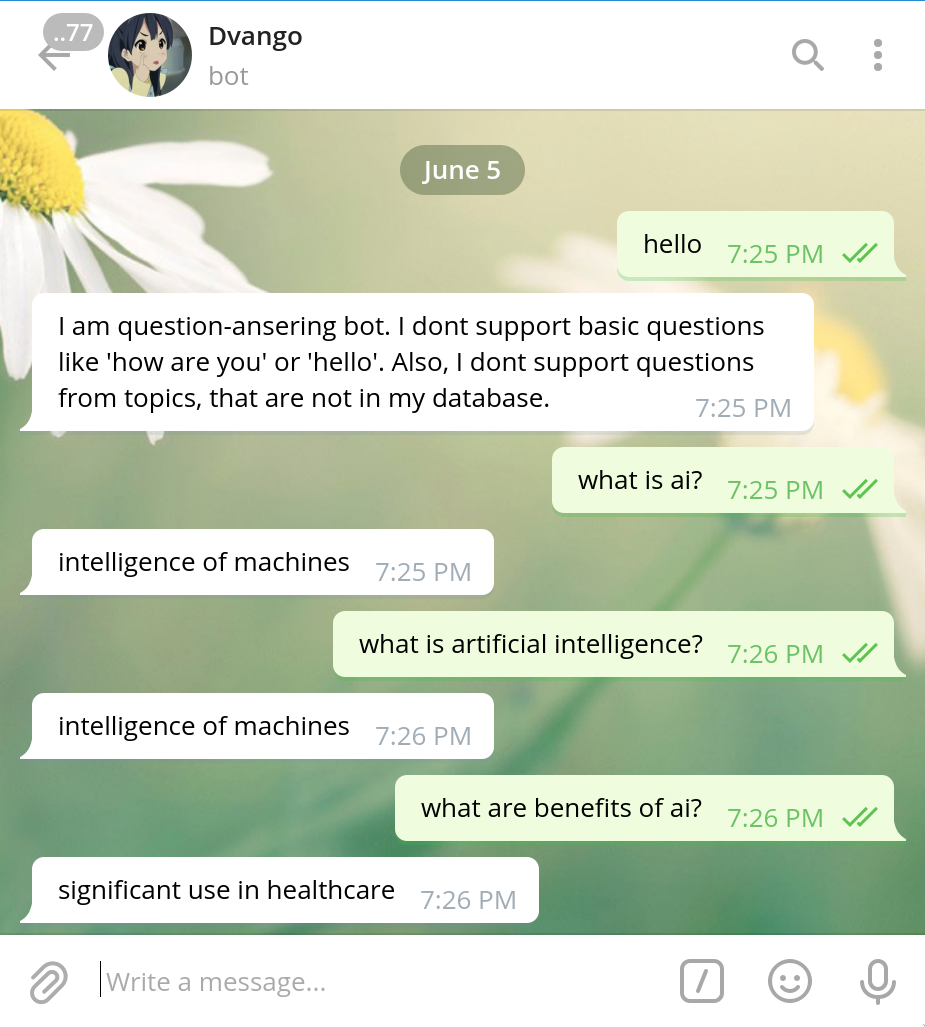
\includegraphics[width=0.75\textwidth]{f1.png}
    \end{figure}
    
    \begin{figure}[H]
        \centering
        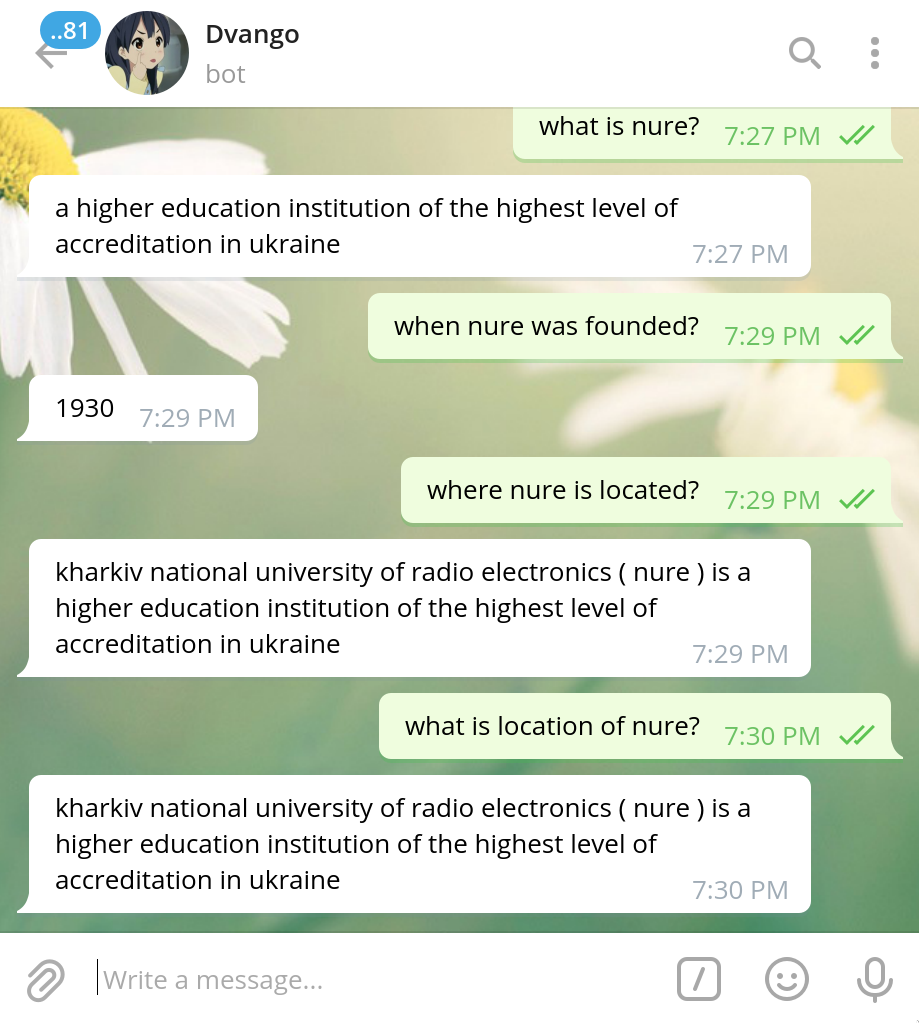
\includegraphics[width=0.75\textwidth]{f2.png}
    \end{figure}

    \begin{figure}[H]
        \centering
        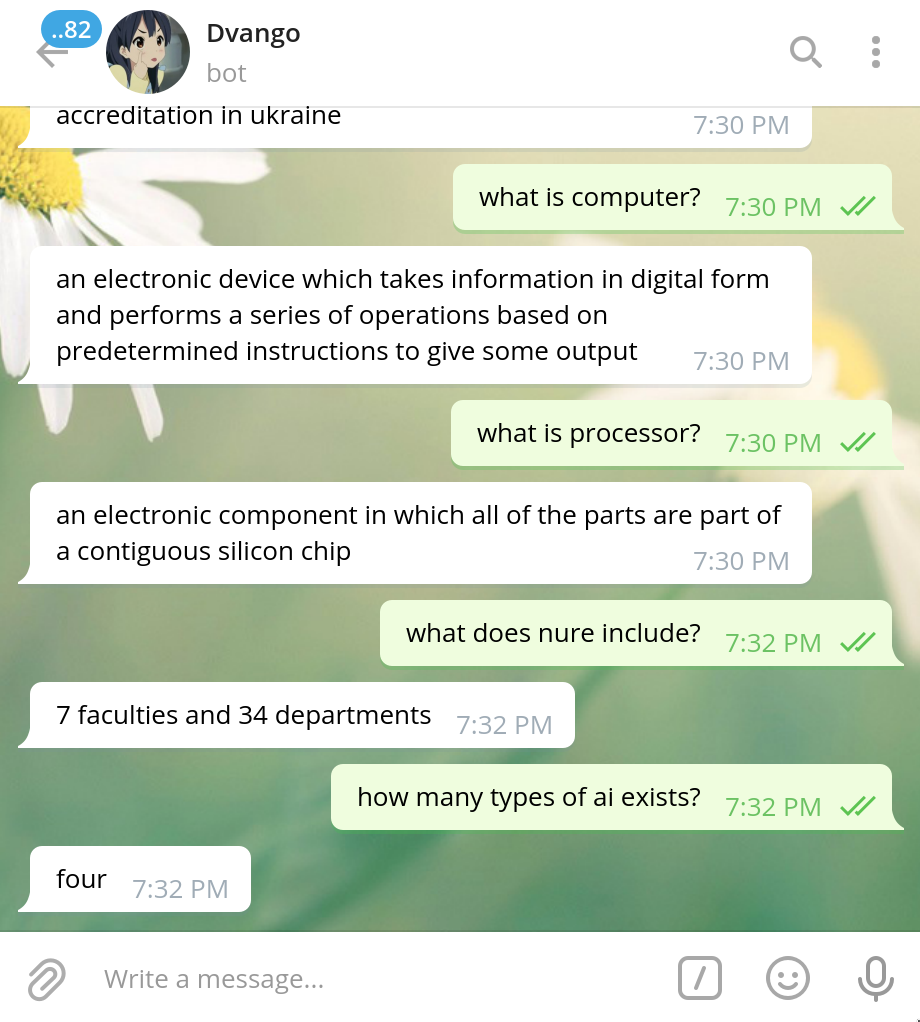
\includegraphics[width=0.75\textwidth]{f3.png}
    \end{figure}
\end{document}


% \begin{figure}[H]
%     \centering
%     \includegraphics[width=0.75\textwidth]{rplot_iris.png}
%     \caption{Графік дерева вибірки Iris з дискретизацією через IG}
%     \label{fig:plot3}
% \end{figure}

% \begin{table}[H]
%     \centering
%     \begin{tabular}{ |c|c|c|c| } 
%      \hline
%      Мова   & \multicolumn{3}{c|}{Метод та датасет} \\ \hline
%             & Iris Thr. & Iris IG & SUSY \\ \hline
%      Python & 0.9333    & 0.9333  & 0.6799 \\ \hline
%      R      & 0.9333    & 0.9777  & 0.6594 \\ 
%      \hline
%     \end{tabular}
%     \caption{Порівняння точності класифікації}
%     \label{tab:t1}
% \end{table}
% \inputminted[breaklines,linenos=true]{scilab}{repl235.txt}
